% ------------------------------------------------------------------------
% bjourdoc.tex for birkjour.cls*******************************************
% ------------------------------------------------------------------------
%%%%%%%%%%%%%%%%%%%%%%%%%%%%%%%%%%%%%%%%%%%%%%%%%%%%%%%%%%%%%%%%%%%%%%%%%%

\documentclass{birkjour}
%
%
% THEOREM Environments (Examples)-----------------------------------------
%
 \newtheorem{thm}{Theorem}[section]
% \newtheorem{cor}[thm]{Corollary}
% \newtheorem{lem}[thm]{Lemma}
% \newtheorem{prop}[thm]{Proposition}
% \theoremstyle{definition}
 \newtheorem{defn}[thm]{Definition}
% \theoremstyle{remark}
% \newtheorem{rem}[thm]{Remark}
% \newtheorem*{ex}{Example}
 \numberwithin{equation}{section}

\usepackage[noadjust]{cite}
\usepackage{amsfonts}
\usepackage{listings}
\usepackage{algorithm}
\usepackage{algorithmic}
\usepackage{booktabs}
\usepackage{float}
\usepackage{caption}

\begin{document}

%-------------------------------------------------------------------------
% editorial commands: to be inserted by the editorial office
%
%\firstpage{1} \volume{228} \Copyrightyear{2004} \DOI{003-0001}
%
%
%\seriesextra{Just an add-on}
%\seriesextraline{This is the Concrete Title of this Book\br H.E. R and S.T.C. W, Eds.}
%
% for journals:
%
%\firstpage{1}
%\issuenumber{1}
%\Volumeandyear{1 (2004)}
%\Copyrightyear{2004}
%\DOI{003-xxxx-y}
%\Signet
%\commby{inhouse}
%\submitted{March 14, 2003}
%\received{March 16, 2000}
%\revised{June 1, 2000}
%\accepted{July 22, 2000}
%
%
%
%---------------------------------------------------------------------------
%Insert here the title, affiliations and abstract:
%


\title[A High-Performance Singularity-Free Rotation Estimator in Geometric Algebra]
 {A High-Performance Singularity-Free Rotation Estimator in Geometric Algebra}

%----------Author 1
\author[Mauricio Cele Lopez Belon]{Mauricio Cele Lopez Belon}
\address{Madrid, España}
\email{mclopez@outlook.com}

%\thanks{This work was completed with the support of our \TeX-pert.}
%----------Author 2
%\author[Jin Wu]{Jin Wu}
%\address{University of Electronic Science and Technology of China, Chengdu, China}
%\email{jin\_wu\_uestc@hotmail.com}

%----------classification, keywords, date
\subjclass{Parallel algorithms 68W10; Clifford algebras, spinors 15A66}

\keywords{Geometric Algebra, Rotation Estimation, Wahba Problem}

\date{October 31, 2016}
%----------additions
%\dedicatory{To my wife}
%%% ----------------------------------------------------------------------

\begin{abstract}

Well known methods for solving the Wahba's problem are formulated in the linear algebra framework, mainly using the SVD or polar decomposition, or in quaternion's framework which leads to solve a max-eigenvalue problem. Those methods are based on well established numerical algorithms which on the other hand are iterative and computationally expensive. Recently, closed form solutions has been proposed based on an analytic formula for solving the roots of the quartic polynomial associated with the eigenvalue problem. Closed form methods are fast but they have singularities i.e., they completely fail on certain input data. In this paper we propose a high-performance, singularity-free estimator of the best quaternion aligning two sets of corresponding vectors i.e., equivalent to Wahba's problem. It is based on a new formulation of the problem in the Geometric Algebra representation of rotations which is isomorphic to Hamilton's quaternions. The proposed method converges in a fixed number of iterations, its performance is competitive with closed form solutions reported in literature and at the same time is free of singularities, robust to noise and simple to implement.

\end{abstract}

%%% ----------------------------------------------------------------------
\maketitle
%%% ----------------------------------------------------------------------
%\tableofcontents
\section{Introduction}

\indent Wahba's problem has been studied for over half a century since 1965 \cite{Wahba1965}. The problem looks for the optimal rotation between two sets of corresponding vectors. Many effective methods have been developed to solving the problem \cite{Arun1987, Horn1987, Mortari1996, Shuster1981, Yang2015} mainly by formulating it in the quaternions framework, which lead us to solve an eigenvalue problem, or by formulating it in the linear algebra framework and using the Singular Value Decomposition (SVD) and recently by formulating it in the Geometric Algebra framework \cite{Perwass2009, Dorst2011} which at some point casts the solution into linear algebra framework and SVD due to the lack of geometric algebra numerical algorithms. More recently, closed form solutions for computing the optimal quaternion has been proposed \cite{Yang2013, Wu2017, Wu2018FA3R, Wu2018FS3R} based on solving the roots of the quartic polynomial associated with the eigenvalue problem with an analytic formula.

Accuracy and speed of most methods have been compared in previous works \cite{Eggert1997, Markley1999, Wu2017} where the trade-off between performance and robustness is assessed. In particular SVD based methods exhibit very good accuracy but low performance and quaternion based methods are in the other end depending on the implementation. Regarding the later methods, the proposed closed form solutions exhibit the best trade-off so far but they have singularities i.e., they completely fail on certain input data.

In this paper we propose a high-performance, singularity-free estimator of the best quaternion aligning two sets of corresponding vectors i.e., equivalent to Wahba's problem. It is based on a new formulation of the problem  in the Geometric Algebra representation of rotations which is isomorphic to Hamilton's quaternions.  The proposed method converge in a fixed number of iterations being is as fast as the closed form solutions reported in literature and at the same time is free of singularities, robust to noise and simple to implement.

In this work we propose a high-performance, singuarity-free method for solving the Wahba's problem. It is based on a maximizing a convex quadratic energy functional, which is equivalent to Wahba's problem, formulated in geometric algebra framework $\mathbb{G}_3$. The proposed method converges in a fixed number of iterations being is as fast as the closed form solutions reported in literature and at the same time is free of singularities and simple to implement.

Applications of Wahba's solutions are diverse from aerospace engineering computation of spacecraft attitude \cite{Wu2017} to mesh deformation in computer graphics \cite{Sorkine2007, Sin2013} for accurate motion construction and restoration \cite{Nieto2012, Perwass2009}. An important characteristic of our method is that it is based almost entirely on symmetric-matrix multiplication so it can be hardware-accelerated using vector instructions or graphics hardware without effort. In engineering fields requiring high-performance vector alignment our method can lower down the time by taking advantage of the AVX (Advanced Vector Extensions) support available in modern microprocessors. Modern matrix packages such as Eigen \cite{Eigen} can produce apropriate AVX instructions automatically. In computer graphics applications our method can lower down the time even more by taking advantage of GPU vector instructions obtaining a performance boost not present in other numerical algorithms.

Few work has been done on studying this problem using geometric algebra. Geometric algebra rotors are closely related to quaternions (quaternion algebra can be regarded as a geometric algebra defined on a set of imaginary basis vectors) we find geometric algebra to be a more natural choice for studying this problem since it is defined over a Euclidean vector space $\mathbb R^3$, where original data is defined. In contrast to previous works we base our formulation on bivectos instead of vectors for the sake of mathematical convenience. Due to mathematical duality of vector and bivectors in $\mathbb{G}_3$ our formulation is also valid for vectors. The implementation of our algorithm does not require any geometric algebra library, we present an implementation based on standard matrix and quaternion library. 

\indent This paper is arranged as follows: Section II introduces the geometric algebra $\mathbb{G}_3$, Section III includes the presentation of our fast rotor estimation algorithm. Section IV demonstrates the experimental results.

\section{Geometric Algebra $\mathbb{G}_3$}

A geometric algebra $\mathbb{G}_3$ is constructed over a real vector space $\mathbb R^3$, with basis vectors $\{e_1, e_2, e_3\}$. The associative geometric product is defined so that the square of any vector is a scalar $a a = a^2 \in \mathbb{R}$. From the vector space $\mathbb R^3$, the geometric product generates the geometric algebra $\mathbb{G}_3$ with elements $\{ X, R, A...\}$ called multivectors.

For a pair of vectors, a symmetric inner product $a \cdot b = b \cdot a$ and antisymmetric outer product $a \wedge b = -b \wedge a$ can be defined implicitly by the geometric product $a b = a \cdot b + a \wedge b$ and $b a = b \cdot a + b \wedge a$. It is easy to prove that $a \cdot b = \frac{1}{2}(a b + b a)$ is scalar, while the quantity $a \wedge b = \frac{1}{2}(a b - b a)$, called a bivector or $2$-vector, is a new algebraic entity that can be visualized as the two-dimensional analogue of a direction, that is, a planar direction. Similar to vectors, bivectors can be decomposed in a bivector basis $\{ e_{12}, e_{13}, e_{23} \}$ where $e_{ij} = e_i \wedge e_j$.

The outer product of three vectors $a \wedge b \wedge c$ generates a $3$-vector also known as the pseudoscalar, because the trivector basis consist of single element $e_{123} = e_1 \wedge e_2 \wedge e_3$. Similarly, the scalars are regarded as $0$-vectors whose basis is the number $1$. It follows that the outer product of $k$-vectors is the completely antisymmetric part of their geometric product: $a_1 \wedge a_2 \wedge ... \wedge a_k = \langle a_1 a_2 ... a_k \rangle_k$ where the angle bracket means $k$-vector part, and $k$ is its grade. The term grade is used to refer to the number of vectors in any exterior product. This product vanishes if and only if the vectors are linearly dependent. Consequently, the maximal grade for nonzero $k$-vectors is $3$. It follows that every multivector $X$ can be expanded into its $k$-vector parts and the entire algebra can be decomposed into $k$-vector subspaces:
\begin{equation*}
\mathbb G_3 = \sum_{k=0}^n{\mathbb{G}^k_3} = \{ X = \sum_{k=0}^n { \langle X \rangle_k } \}
\end{equation*}
This is called a \emph{grading} of the algebra. 

Reversing the order of multiplication is called reversion, as expressed by $(a_1 a_2 ... a_k)\tilde{} = a_k ... a_2 a_1$ and $(a_1 \wedge a_2 \wedge ... \wedge a_k)\tilde{} = a_k \wedge ... \wedge a_2 \wedge a_1$, and the reverse of an arbitrary multivector is defined by $\tilde{X} = \sum_{k=0}^n { \langle \tilde{X} \rangle_k }$.

Rotations are even grade multivectors known as rotors. We denote the subalgebra of rotors as $\mathbb{G}^{+}_3$. A rotor $R$ can be generated as the geometric product of an even number of vectors. A reflection of any $k$-vector $X$ in a plane with normal $n$ is expressed as the sandwitch product $(-1)^k n X n$. The most basic rotor $R$ is defined as the product of two unit vectors $a$ and $b$ with angle of $\frac{\theta}{2}$. The rotation plane is the bivector $B = \frac{a \wedge b}{\| a \wedge b \|}$.
\begin{equation}
a b = a \cdot b + a \wedge b = \cos\left( \frac{\theta}{2} \right) + B \sin\left( \frac{\theta}{2} \right).
\end{equation}
Rotors act on all $k$-vectors using the sandwitch product $X' = R X \tilde R$, where $\tilde R$ is the reverse of $R$ and can be obtained by reversing the order of all the products of vectors.

\section{Geometric Algebra Rotor Estimation}

Given two sets of $n$ corresponding bivectors $P = \{p_j\}_{j=1}^n$ and $Q = \{q_j\}_{j=1}^n$, we attempt to maximize the following energy function:
\begin{eqnarray}
	E(R) = \max_{R \in \mathbb{G}^{+}_3 } \sum_j { c_{j} \|p_j + \tilde R q_i R \|^2 }\\
	s.t. \ R \tilde R = 1
\end{eqnarray}
where $\{c_{j}\}_{j=1}^n$ are scalar weights such that $\sum_j^n{c_j} = 1$. It is a non-linear quadratic maximization problem with a non-linear constraint in $R$. Notice that the term $\|p_j + \tilde R q_i R\|^2$ is dual to the traditional least squares error $\|q_j - R p_j \tilde R\|^2$. Duality in the sense that the optimal $R$ is a critical point of both energies.
Notice also that $p_j + \tilde R q_i R$ is equivalent to $R p_j + q_j R$ by multiplying by $R$ on the left and using the fact that $R \tilde R = 1$. The equivalent problem is:
\begin{eqnarray}
	E(R) = \max_{R \in \mathbb{G}^{+}_3 } \sum_j { c_{j} \|R p_j + q_j R\|^2 }\\
	s.t. \ R \tilde R = 1
\end{eqnarray}
which is a linear maximization problem with a non-linear constraint in $R$.

We define the commutator product of two bivectors $p_j$ and $q_j$ as $p_j \times q_j = \frac{1}{2}(p_j q_j - q_j p _j)$. The commutator product of bivectors in $\mathbb{G}_3$  can be interpreted as a cross-product of bivectors in the sense that the resulting bivector $B = p_j \times q_j$ is orthogonal to both $p_j$ and $q_j$. The commutator product allow us to define the geometric product of two bivectors as $A B = A \cdot B + A \times B$. Recall that the inner product of bivectors is not the same as the inner product of vectors, since the square of bivectors is negative, the inner product of bivectors has the opposite sign e.g., $(a e_{12} + b e_{13} + c e_{23}) \cdot (d e_{12} + e e_{13} + f e_{23}) = -a d - b e - c f$.

For a pair of unit bivectors, $A$ and $B$, the rotor $R$ aligning them can be defined as $R = A \frac{(A + B)}{\|A + B\|}$. Defining the unit bivector $C = \frac{A + B}{\|A + B\|}$ the rotor $R$ is also $R = A C = w + L$ where $w = A \cdot C = \cos(\theta/2)$ and $L = A \times C = \sin(\theta/2) \frac{A \times B}{\|A \times B\|}$.

The constraint $R p_j + q_j R$ can be rewriten as $(w + L) p_j  + q_j (w + L)$. Expanding the geometric product of bivectors in terms of the inner product and the communtator product we get:
\begin{eqnarray}
	w  (p_j + q_j) + L \cdot (p_j + q_j)  + (q_j - p_j) \times L
\end{eqnarray}

In matrix language we can define the following matrix system $M_j R = 0$:
\begin{eqnarray}
	M_j R =
	\left[\begin{array}{cc}
		0      &       -s_j^T \\
		s_j    &   \left[ d_j \right]_\times \\
	\end{array}\right]
	\left[\begin{array}{c} 
		w \\
		L
	\end{array}\right] = 
	\left[\begin{array}{c}
		-s_j^T L \\
		w s_j + d_j \times L 
	\end{array}\right]\\
	d_j = q_j - p_j \ \ s_j = p_j + q_j
\end{eqnarray}
where $d_j$ and $s_j$ are $3 \times 1$ column vectors holding bivector's coefficients, $M_j$ is a skew-symmetric $4\times 4$ real matrix, so that $M_j^T = -M_j$. The rotor $R$ is represented as $4 \times 1$ column vector made of the scalar $w$ and the $3 \times 1$ column vector $L$ holding the bivector's components. The $3\times 3$ matrix $\left[ d_j \right]_\times$ is representing the skew-symmetric cross-product matrix as usually defined for vectors in $\mathbb R^3$.

Let define the function $F^j$ representing the linear transformation:
\begin{eqnarray*}
F^j = \sqrt{c_j} M_j R\\
\end{eqnarray*}

Let $F$ be a column vector of $n$ stacked functions $F^j$
\begin{eqnarray*}
F = \left[\begin{array}{c}F^1 \\ \vdots \\ F^n\end{array}\right]
\end{eqnarray*}
 such that the energy $E(R)$ can be expressed as matrix product
\begin{eqnarray*}
E(R) = F^T F =
\left[\begin{array}{ccc}F^{1T} & \cdots & F^{nT}\end{array}\right]
\left[\begin{array}{c}F^1 \\ \vdots \\ F^n\end{array}\right]
\end{eqnarray*}

We can express $E(R)$ as the following quadratic form:
\begin{eqnarray}
E(R) = \max_R R^T M R\\
s.t. \ R^T R = 1
\end{eqnarray}
where $M = \sum_j^n { c_j M_j^T M_j}$. Note that since $M_j$ is skew-symmetric, the product $M_j^T M_j$ is symmetric and positive semi-definite.
Consequently the matrix $M$ is also symmetric positive semi-definite. It follows that all eigenvalues of $M$ are real and $\lambda_i \geq 0$.
\begin{eqnarray}
	M_j^T M_j = 
	\left[\begin{array}{cc}
		\| s_j \|^2       &         (s_j \times d_j)^T \\
		s_j \times d_j  &    s_j s_j^T - \left[ d_j \right]^2_\times \\
	\end{array}\right]\\
	d_j = q_j - p_j \ \ s_j = p_j + q_j
\end{eqnarray}

By the spectral theorem the maximizer of $E(R)$ is the eigenvector of $M$ associated with the largest eigenvalue which is a positive number.

\section{Convexity}

The convexity of the energy $E(R)$ can be proof by showing that its Hessian matrix of second partial derivatives is positive semi-definite. The Hessian matrix of $E(R)$ is $\frac{\partial^2 E(R)}{\partial R} = \sum_j^n { c_j M_j^T M_j}$ which is symmetric, moreover since $M_j$ is skew-symmetric matrix, the product $M_j^T M_j$ is symmetric positive semi-definite. Then follows that $\sum_j^n { c_j M_j^T M_j}$ is positive semi-definite and therefore convex, provided that the sum of weights is convex i.e., $\sum_j^n { c_j } = 1$.

\section{Optimal Quaternion using 4D Geometric Algebra}

The most time consuming task of the estimation is to compute the eigenvector of $M$ associated with the greatest eigenvalue. Sound numerical algorithms for computing eigenvectors of a real symmetric matrix are SVD, QR factorization and Jacobi iteration among others. However those algorithms finds all eigenvectors of a matrix. In this section we show how to find the largest eigenvalue and its corresponding eigenvector i.e., the required quaternion, using the 4D Geometric Algebra $ \mathbb{G}_4$ which is efficient, accurate and suitable for high performance applications.

Let us define four vectors $\textbf m_1$, $\textbf m_2$, $\textbf m_3$, $\textbf m_4$ corresponding to the columns of matrix $M$:
\begin{eqnarray*}
	M = \sum_j^n { c_j M_j^T M_j} =
	\left[\begin{array}{cccc}
		\\
		\textbf m_1 & \textbf m_2 & \textbf m_3 & \textbf m_4 \\
		\\
	\end{array}\right]
\end{eqnarray*}

The matrix system that we want to solve is $M R = \lambda R$ for $\lambda$ corresponding to the largest eigenvalue of $M$ and the corresponding $R$. We can write the system in the following form:
\begin{eqnarray}
	\left[\begin{array}{cccc}
		\\
		\textbf m_1 - \lambda e_1 & \textbf m_2 - \lambda e_2 & \textbf m_3 - \lambda e_3 & \textbf m_4- \lambda e_4 \\
		\\
		\\
	\end{array}\right]
	\left[\begin{array}{c} 
		w \\
		L_1\\
		L_2\\
		L_3
	\end{array}\right] = 	
	\left[\begin{array}{c} 
		0 \\
		0 \\
		0 \\
		0
	\end{array}\right]
	\label{eqn:eigensystem}
\end{eqnarray}

The matrix in equation~\ref{eqn:eigensystem}, called \emph{characteristic matrix}, is singular ie., the vectors $(\textbf m_1 - \lambda e_1)$, $(\textbf m_2 - \lambda e_2)$, $()\textbf m_3 - \lambda e_3)$ and $()\textbf m_4- \lambda e_4)$ are linearly dependent (the rank of the matrix is $3$). It follows that its outer product must be zero:
\begin{eqnarray}
(\textbf m_1 - \lambda e_1)\wedge(\textbf m_2 - \lambda e_2)\wedge(\textbf m_3 - \lambda e_3)\wedge(\textbf m_4- \lambda e_4) = 0
	\label{eqn:characteristic_outer_product}
\end{eqnarray}

Which is called the \emph{charactetistic outer porduct} and is equivalent to the characteristic polynomial $P(\lambda) = det(M - \lambda I)$. We can find the largest root of the polynomial using Newton-Raphson method $\lambda_{i+1} = \lambda_i - P(\lambda) / P'(\lambda)$. For the sake of completeness we show the first derivative of \ref{eqn:characteristic_outer_product}:
\begin{eqnarray*}
P'(\lambda) = 
- e_1\wedge(\textbf m_2 - \lambda e_2)\wedge(\textbf m_3 - \lambda e_3)\wedge(\textbf m_4- \lambda e_4)\\
- (\textbf m_1 - \lambda e_1)\wedge e_2\wedge(\textbf m_3 - \lambda e_3)\wedge(\textbf m_4- \lambda e_4)\\
- (\textbf m_1 - \lambda e_1)\wedge(\textbf m_2 - \lambda e_2)\wedge e_3\wedge(\textbf m_4- \lambda e_4)\\
- (\textbf m_1 - \lambda e_1)\wedge(\textbf m_2 - \lambda e_2)\wedge(\textbf m_3 - \lambda e_3)\wedge e_4
\end{eqnarray*}

We found that $Trace(M)$ is a robust guess for Newton-Raphson iteration because it is larger than the largest eigenvalue and is also close enough to converge in few iterations.

Following \cite{DeKeninck2019} we solve the system~\ref{eqn:eigensystem} using outer products. For a linear system $A \textbf x = b$ the authors in \cite{DeKeninck2019} defines $N$ linear equations of the form $A^T_j \textbf x = b_j$ each of which corresponds to a dual hyper-plane of the form $\textbf a_j \equiv A_j - b_j e_0$ where the solution $\textbf x$ must lie on. The $e_0$ is an \emph{homogeneous} basis vector needed for enabling projective geometry, enlarging the base space to $N+1$, which interpretation is to be the offset of the hyper-plane. So solution of the linear system is the intersection of $N$ dual hyper-planes, which is given by its outer product.
\begin{eqnarray}
\alpha (\textbf x + e_0)^* = \textbf a_1 \wedge \textbf a_2 \wedge ... \wedge \textbf a_N
\end{eqnarray}

Where the symbol $^*$ is the dual operator of the $N+1$ space and $\alpha$ is a weight factor. After taking the dual of $\alpha (\textbf x + e_0)^*$ and divide by the coefficient of $e_0$ (which is $\alpha$), the solution $\textbf x$ can be read off the coefficients of the $1$-vector.

We know that the null space of $(M - \lambda I)$ is of rank one. Algebraically this means that one of its column vectors is redundant i.e., it can be written in term of the others. In linear algebra this means that the system has infinitely many solutions. The geometric interpretation is that all hyper-planes intersect in a line passing through the origin. Since all solutions lie on the same line and they only differ by a scaling term, a particular solution can be found by fixing the scale. Actually, it is enough to constrain the scale of a single hyper-plane. The homogeneous component $e_0$ can be interpreted as scale of solution (instead of hyper-plane's offset as in \cite{DeKeninck2019}) since it affects only that aspect of the solution. In linear algebra language it is equivalent to set one value at the right hand side of \ref{eqn:eigensystem}, however that system can't be solved in linear algebra because it requires to invert a singular matrix.

We define the dual hyper-planes passing through the origin as:
\begin{eqnarray}
   \textbf a_i \equiv \textbf m_i - \lambda e_i
\end{eqnarray}

Although in most cases it is enough to set the scale of a single hyper-plane go get a solution it is inconvenient to do so, as will be explained in Section~\ref{section:robustness}. It is more robust to set the scale of all hyper-planes to some $\gamma \neq 0$ which is a scalar value. Intersection can then be found by taking the outer product as:
\begin{eqnarray}
\alpha (\textbf x + 1)^* = (\textbf a_1 + \gamma) \wedge  (\textbf a_2 + \gamma) \wedge  (\textbf a_3  + \gamma) \wedge (\textbf a_4 + \gamma)
\label{eqn:hyperplanes_intersection}
\end{eqnarray}

Distributing the outer product and keeping the terms of grade-$3$ we get:
\begin{eqnarray}
\alpha (\textbf x + 1)^* =  \gamma (\textbf a_1 \wedge \textbf a_3 \wedge \textbf a_4
+ \textbf a_1 \wedge \textbf a_2 \wedge \textbf a_4
+ \textbf a_1 \wedge \textbf a_2 \wedge \textbf a_3
+ \textbf a_2 \wedge \textbf a_3 \wedge \textbf a_4)
\end{eqnarray}

Here the symbol $^*$ is the dual operator of the $4$D space (not $5$D as in \cite{DeKeninck2019} which allow us to be more efficient) and $\alpha$ is a weight factor. After taking the dual of $\alpha (\textbf x + 1)^*$ the eigenvector $\textbf x$ can be read off the coefficients of the $1$-vector. Notice that solution needs to be normalized.


\section{Robustness and Singularities}
\label{section:robustness}

As stated before, setting the scale of a single hyperplane is enough to get a valid eigenvector in most cases. However, the choice of which hyper-plane to constraint is problematic. For instance,  assuming input vectors without noise, constraining the hyperplane corresponding to the $w$ component of the rotor won't work when the angle of rotation is $\pi$ because $w = \cos(\pi/2)$ in that case. Similarly, constraining one of the hyper-planes corresponding to $L_1$, $L_4$ or $L_3$ won't work when the angle of rotation is $0$ or $4 \pi$, etc. So it is complex task to avoid all problematic situations. By constraining all hyper-planes as in \ref{eqn:hyperplanes_intersection} our geometric algebra method does not suffer from any of those singularities.

Some of the above mentioned singularities are present in classic methods such as QUEST \cite{Shuster1981} and FOAM \cite{Markley1993} but also on methods derived from those, including recent descendants based on analytic formulas \cite{Yang2013, Wu2016, Wu2017, Wu2018FA3R, Wu2018FS3R}. All those methods are based on finding the eigenvector corresponding to largest eigenvalue of Davenport's matrix. Since it is an indefinite matrix, some eigenvalues are positive and some negative, the Newton-Raphson can fail to find the max eigenvalue (which can be negative). So significant effort has been put on finding fast and robust analytic solutions to the quartic polynomial but no advances has been made on improving robustness on finding the associated eigen-vector.

\section{Optimal Computation of M}

The symmetric matrix $M_j^T M_j$ has a simple form:

\begin{eqnarray*}
	M_j^T M_j = 
	\left[\begin{array}{cc}
		\| s_j \|^2        &         (s_j \times d_j)^T \\
		s_j \times d_j  &    s_j s_j^T - d_j d_j^T + \| d_j \|^2 I \\
	\end{array}\right]\\
	d_j = q_j - p_j \ \ s_j = p_j + q_j
\end{eqnarray*}

In terms of $p_j$ and $q_j$ it is:

\begin{eqnarray*}
	M_j^T M_j = 2
	\left[\begin{array}{cc}
		p_j^T q_j       &         (p_j \times q_j)^T \\
		p_j \times q_j  &    p_j q_j^T + q_j p_j^T - p_j^Tq_j I_{3\times3} \\
	\end{array}\right]
    + (\| p_j \|^2 + \| q_j \|^2) I_{4\times4}\\
\end{eqnarray*}
All terms of the matrix $M_j^T M_j$ can be derived from the matrix $B = p_j q_j^T$ plus the quantiry $\| p_j \|^2 + \| q_j \|^2$. Since $M_j^T M_j$ is symmetric, only $10$ out of $16$ elements need to be actually computed. Notice that the trace of $M_j^T M_j$ is $Tr(M_j^T M_j) = 4 \|p_j\|^2 + 4 \|q_j\|^2$ and $Tr(H) = 4 \sum_j {(\|p_j\|^2 + \|q_j\|^2)}$.

\section{Algorithms}

The pseudo-code of proposed method is shown in Algorithm~\ref{alg:FastRotorEstimation}. 

\begin{algorithm}
\begin{algorithmic}[1]
\REQUIRE {$P = \{p_{j}\}_{j=1}^n, Q = \{q_{j}\}_{j=1}^n, C = \{c_{j}\}_{j=1}^n$}
\STATE{$S = B = 0, \gamma = 1$}
\FOR{$j = 1$ \TO $n$}
\STATE{$S = S + c_j (p_j \cdot p_j + q_j \cdot q_j)$}
\STATE{$B = B + c_j p_j q_j^T$}
\ENDFOR
\STATE{$\textbf m_1 = (S + Tr(B)) e_1 + (B_{12} - B_{21}) e_2 + (B_{20} - B_{02}) e_3 + (B_{01} - B_{10}) e_4$}
\STATE{$\textbf m_2 = (B_{12} - B_{21})e_1 + 2 (B_{00} + S - Tr(B)) e_2 + (B_{01} + B_{10}) e_3 + (B_{20} + B_{02}) e_4$}
\STATE{$\textbf m_3 = (B_{20} - B_{02})e_1 + (B_{01} + B_{10}) e_2 + 2 (B_{11} + S - Tr(B)) e_3 + (B_{12} + B_{21}) e_4$}
\STATE{$\textbf m_3 = (B_{01} - B_{10})e_1 + (B_{20} + B_{02} ) e_2 + (B_{12} + B_{21}) e_3 + 2 (B_{22} + S - Tr(B)) e_4$}
\COMMENT{Newton-Raphson}
\STATE{$\lambda_0 = 7 S - 3 Tr(B)$}
\REPEAT
\STATE{$\lambda_{i+1} = \lambda_i - P(\lambda_i) / P'(\lambda_i)$}
\UNTIL{$\|\lambda_{i+1} - \lambda_i\| < \epsilon$}
\STATE{$\textbf a_1 = \textbf m_1 - \lambda e_1$
}
\STATE{$\textbf a_2 = \textbf m_2 - \lambda e_2$
}
\STATE{$\textbf a_3 = \textbf m_3 - \lambda e_3$
}
\STATE{$\textbf a_4 = \textbf m_4 - \lambda e_4$
}
\STATE{$\textbf X = \gamma (\textbf a_1 \wedge \textbf a_3 \wedge \textbf a_4
	+ \textbf a_1 \wedge \textbf a_2 \wedge \textbf a_4
	+ \textbf a_1 \wedge \textbf a_2 \wedge \textbf a_3
	+ \textbf a_2 \wedge \textbf a_3 \wedge \textbf a_4)$}
\STATE{$R = normalize( \langle \textbf X^* \rangle_1 )$}
\RETURN { $R(0) + R(1) e_{12} + R(2) e_{13} + R(3) e_{23}$ }
\end{algorithmic}
\caption{Fast Rotor Estimation}\label{alg:FastRotorEstimation}
\end{algorithm}
An optimized C++ code using the Eigen library \cite{Eigen} can be found in Listing~\ref{lst:cppcode}.

\section{Comparisons}

We select several representative methods e.g. FLAE \cite{Wu2017}, SVD \cite{Horn1987} and QUEST \cite{Shuster1981} to implement the algorithm. The Eigen library \cite{Eigen} is employed to implement the SVD and QUEST. Another version of QUEST using the Newton iteration is also added for comparison. The tests are ran on a MacBook Pro 13' 2017 computer with the CPU of Intel 3.1GHz 4-core i5. The Visual Studio 2019 C++ compiler is used in our experiments. %The results are listed below (Table \ref{tab:roll}, \ref{tab:pitch}, \ref{tab:yaw}):

% \begin{table} [H]
% \centering
% \begin{minipage}[b]{1.0\textwidth}
% \caption{Roll RMSE (deg)}  
%  \label{tab:roll}
% \resizebox{1.0\textwidth}{!}{ 
% \begin{tabular}{cccccc}
% \toprule
% {Case}&{Proposed}&{SVD Horn 1987}&{FLAE 2017}&{QUEST Eigen 1981}&{QUEST Newton 1981}\\
% \midrule
% {1}&{$4.9426 \times 10^{-04}$}&{$4.3068 \times 10^{-05}$}&{$4.3068 \times 10^{-05}$}&{$4.3068 \times 10^{-05}$}&{$4.3068 \times 10^{-05}$}\\
% {2}&{$3.3673 \times 10^{-04}$}&{$5.9781 \times 10^{-05}$}&{$5.9781 \times 10^{-05}$}&{$5.9781 \times 10^{-05}$}&{$5.9781 \times 10^{-05}$}\\
% {3}&{$2.4912 \times 10^{+00}$}&{$4.3420 \times 10^{-01}$}&{$4.3420 \times 10^{-01}$}&{$4.3420 \times 10^{-01}$}&{$4.3420 \times 10^{-01}$}\\
% {4}&{$3.4014 \times 10^{+00}$}&{$5.9978 \times 10^{-01}$}&{$5.9978 \times 10^{-01}$}&{$5.9978 \times 10^{-01}$}&{$5.9978 \times 10^{-01}$}\\
% {5}&{$3.9992 \times 10^{+00}$}&{$4.3545 \times 10^{-01}$}&{$2.1560 \times 10^{+01}$}&{$4.3545 \times 10^{-01}$}&{$4.3649 \times 10^{-01}$}\\
% {6}&{$4.9857 \times 10^{-02}$}&{$4.9792 \times 10^{-03}$}&{$4.9792 \times 10^{-03}$}&{$4.9792 \times 10^{-03}$}&{$4.9792 \times 10^{-03}$}\\
% {7}&{$8.7731 \times 10^{-02}$}&{$8.1146 \times 10^{-03}$}&{$8.1146 \times 10^{-03}$}&{$8.1146 \times 10^{-03}$}&{$8.1146 \times 10^{-03}$}\\
% {8}&{$3.4008 \times 10^{+02}$}&{$5.9402 \times 10^{+01}$}&{$5.9402 \times 10^{+01}$}&{$5.9402 \times 10^{+01}$}&{$5.9402 \times 10^{+01}$}\\
% {9}&{$5.3870 \times 10^{+02}$}&{$7.7637 \times 10^{+01}$}&{$7.7638 \times 10^{+01}$}&{$7.7637 \times 10^{+01}$}&{$7.7637 \times 10^{+01}$}\\
% {10}&{$1.3513 \times 10^{+01}$}&{$1.4641 \times 10^{+00}$}&{$1.5824 \times 10^{+00}$}&{$1.4641 \times 10^{+00}$}&{$1.4641 \times 10^{+00}$}\\
% {11}&{$1.9366 \times 10^{+01}$}&{$2.0427 \times 10^{+00}$}&{$2.9300 \times 10^{+00}$}&{$2.0427 \times 10^{+00}$}&{$2.0427 \times 10^{+00}$}\\
% {12}&{$1.2517 \times 10^{+01}$}&{$2.0712 \times 10^{+00}$}&{$1.7328 \times 10^{+01}$}&{$2.0712 \times 10^{+00}$}&{$3.3679 \times 10^{+01}$}\\
% \bottomrule
% \end{tabular}}
% \end{minipage}

% \begin{minipage}[b]{1.0\textwidth}
% \caption{Pitch RMSE (deg)}  
%  \label{tab:pitch}
% \resizebox{1.0\textwidth}{!}{ 
% \begin{tabular}{cccccc}
% \toprule
% {Case}&{Proposed}&{SVD Horn 1987}&{FLAE 2017}&{QUEST Eigen 1981}&{QUEST Newton 1981}\\
% \midrule
% {1}&{$4.0745 \times 10^{-04}$}&{$4.0500 \times 10^{-05}$}&{$4.0500 \times 10^{-05}$}&{$4.0500 \times 10^{-05}$}&{$4.0500 \times 10^{-05}$}\\
% {2}&{$4.1322 \times 10^{-04}$}&{$5.3106 \times 10^{-05}$}&{$5.3106 \times 10^{-05}$}&{$5.3106 \times 10^{-05}$}&{$5.3106 \times 10^{-05}$}\\
% {3}&{$4.0623 \times 10^{+00}$}&{$4.0205 \times 10^{-01}$}&{$4.0205 \times 10^{-01}$}&{$4.0205 \times 10^{-01}$}&{$4.0205 \times 10^{-01}$}\\
% {4}&{$6.0567 \times 10^{+00}$}&{$5.2600 \times 10^{-01}$}&{$5.2600 \times 10^{-01}$}&{$5.2600 \times 10^{-01}$}&{$5.2600 \times 10^{-01}$}\\
% {5}&{$2.4391 \times 10^{+00}$}&{$3.9376 \times 10^{-01}$}&{$1.1799 \times 10^{+01}$}&{$3.9376 \times 10^{-01}$}&{$3.9469 \times 10^{-01}$}\\
% {6}&{$3.6311 \times 10^{-04}$}&{$4.0168 \times 10^{-05}$}&{$4.0168 \times 10^{-05}$}&{$4.0168 \times 10^{-05}$}&{$4.0168 \times 10^{-05}$}\\
% {7}&{$6.2653 \times 10^{-04}$}&{$5.3300 \times 10^{-05}$}&{$5.3300 \times 10^{-05}$}&{$5.3300 \times 10^{-05}$}&{$5.3300 \times 10^{-05}$}\\
% {8}&{$4.3060 \times 10^{+00}$}&{$3.6817 \times 10^{-01}$}&{$3.6817 \times 10^{-01}$}&{$3.6817 \times 10^{-01}$}&{$3.6817 \times 10^{-01}$}\\
% {9}&{$5.9480 \times 10^{+00}$}&{$4.5583 \times 10^{-01}$}&{$4.5583 \times 10^{-01}$}&{$4.5583 \times 10^{-01}$}&{$4.5583 \times 10^{-01}$}\\
% {10}&{$4.3860 \times 10^{-04}$}&{$5.8427 \times 10^{-05}$}&{$5.8427 \times 10^{-05}$}&{$5.8427 \times 10^{-05}$}&{$5.8432 \times 10^{-05}$}\\
% {11}&{$4.3787 \times 10^{-04}$}&{$5.7149 \times 10^{-05}$}&{$5.7150 \times 10^{-05}$}&{$5.7149 \times 10^{-05}$}&{$5.7146 \times 10^{-05}$}\\
% {12}&{$2.6414 \times 10^{+00}$}&{$4.8955 \times 10^{-01}$}&{$3.9323 \times 10^{+00}$}&{$4.8955 \times 10^{-01}$}&{$4.8405 \times 10^{+00}$}\\
% \bottomrule
% \end{tabular}}
% \end{minipage}

% \begin{minipage}[b]{1.0\textwidth}
% \caption{Yaw RMSE (deg)}  
%  \label{tab:yaw}
% \resizebox{1.0\textwidth}{!}{ 
% \begin{tabular}{cccccc}
% \toprule
% {Case}&{Proposed}&{SVD Horn 1987}&{FLAE 2017}&{QUEST Eigen 1981}&{QUEST Newton 1981}\\
% \midrule
% {1}&{$8.3214 \times 10^{-04}$}&{$4.2976 \times 10^{-05}$}&{$4.2976 \times 10^{-05}$}&{$4.2976 \times 10^{-05}$}&{$4.2976 \times 10^{-05}$}\\
% {2}&{$4.6383 \times 10^{-04}$}&{$4.8484 \times 10^{-05}$}&{$4.8484 \times 10^{-05}$}&{$4.8484 \times 10^{-05}$}&{$4.8484 \times 10^{-05}$}\\
% {3}&{$3.9084 \times 10^{+00}$}&{$4.3773 \times 10^{-01}$}&{$4.3773 \times 10^{-01}$}&{$4.3773 \times 10^{-01}$}&{$4.3773 \times 10^{-01}$}\\
% {4}&{$2.4989 \times 10^{+00}$}&{$4.8366 \times 10^{-01}$}&{$4.8366 \times 10^{-01}$}&{$4.8366 \times 10^{-01}$}&{$4.8366 \times 10^{-01}$}\\
% {5}&{$1.9721 \times 10^{+00}$}&{$2.5312 \times 10^{-01}$}&{$1.5349 \times 10^{+01}$}&{$2.5312 \times 10^{-01}$}&{$2.5373 \times 10^{-01}$}\\
% {6}&{$2.2129 \times 10^{-04}$}&{$3.6325 \times 10^{-05}$}&{$3.6325 \times 10^{-05}$}&{$3.6325 \times 10^{-05}$}&{$3.6325 \times 10^{-05}$}\\
% {7}&{$3.5209 \times 10^{-04}$}&{$4.9660 \times 10^{-05}$}&{$4.9660 \times 10^{-05}$}&{$4.9660 \times 10^{-05}$}&{$4.9660 \times 10^{-05}$}\\
% {8}&{$2.7013 \times 10^{+00}$}&{$3.9770 \times 10^{-01}$}&{$3.9770 \times 10^{-01}$}&{$3.9770 \times 10^{-01}$}&{$3.9770 \times 10^{-01}$}\\
% {9}&{$4.9757 \times 10^{+00}$}&{$4.9710 \times 10^{-01}$}&{$4.9710 \times 10^{-01}$}&{$4.9710 \times 10^{-01}$}&{$4.9710 \times 10^{-01}$}\\
% {10}&{$5.5605 \times 10^{-04}$}&{$6.1117 \times 10^{-05}$}&{$6.1114 \times 10^{-05}$}&{$6.1117 \times 10^{-05}$}&{$6.1118 \times 10^{-05}$}\\
% {11}&{$4.7411 \times 10^{-04}$}&{$6.0821 \times 10^{-05}$}&{$6.0831 \times 10^{-05}$}&{$6.0821 \times 10^{-05}$}&{$6.0820 \times 10^{-05}$}\\
% {12}&{$3.3917 \times 10^{+00}$}&{$3.1503 \times 10^{-01}$}&{$2.8467 \times 10^{+00}$}&{$3.1503 \times 10^{-01}$}&{$6.1232 \times 10^{+00}$}\\
% \bottomrule
% \end{tabular}}
% \end{minipage}
% \end{table}
% In these tables, the Euler angles i.e. roll, pitch and yaw angles are listed for comparisons. The root mean-squared error (RMSE) is presented to describe the difference of accuracy. It is observed that the proposed algorithm has worse accuracy than that from the conventional Wahba's solutions. The time consumption is summarized in Figure \ref{fig:time}. We can also see that the loss of accuracy well worth the computation time. The computation time here from the proposed approach is almost 50\% of that of the known best algorithm FLAE.


% \begin{figure}[H]
% \centering
% 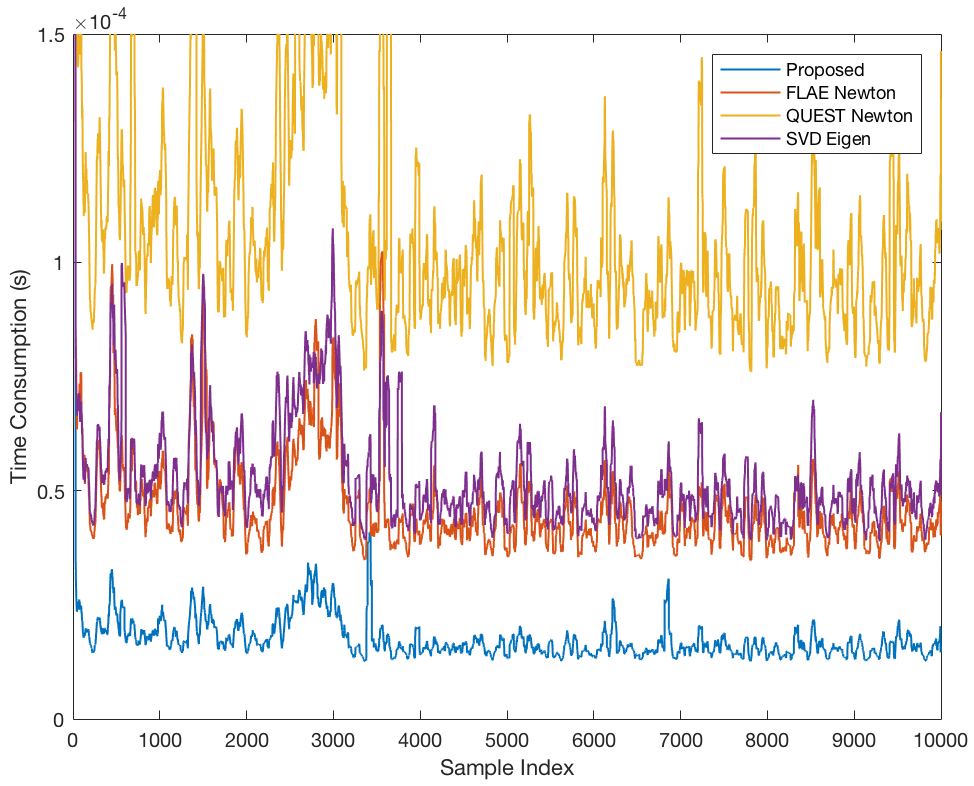
\includegraphics[width=1.0\textwidth]{time.jpg}
% \caption{Execution time consumption of various algorithms.}
% \label{fig:time}
% \end{figure}

\section{Conclusion}
In this paper, we solve the problem of estimating the best rotation for the alignment of two sets of corresponding 3D vectors. It is based on solving the linear equations derived from the formulation of the problem in Geometric Algebra. The method is fast, robust to noise, accurate and simpler than most other methods. Experimental validation of the performance of the proposed algorithm is presented. The results show that the slightly losing accuracy of the proposed method is well worth the huge advance in execution time consumption. For many applications the vector datasets are very huge i.e. the computation time would be more important than slight change of accuracy. Therefore, we hope that the proposed algorithm would be of benefit to such applications.


\section{C++ code}

\begin{lstlisting}[language=C++, caption=C++ code for rotor estimation, basicstyle=\tiny, keywordstyle=\bfseries, label=lst:cppcode, morekeywords={Matrix4d,Matrix3d,Vector4d,Vector3d,Quaterniond,sqrt,__m256d,__m128d}]
Quaterniond GAFastRotorEstimator(
    const vector<Vector3d>& P, 
    const vector<Vector3d>& Q, 
    const vector<double>& w)
{
  array<double, 10> H;
  Matrix3d Sx;
  Vector3d S;
  double wj;
  const size_t N = P.size();
  Sx.setZero();
  S.setZero();
  for (size_t j = 0; j < N; ++j) {
    wj = w[j];
    const Vector3d& Qj = Q[j];
    const Vector3d& Pj = P[j];
    S.noalias() += wj * (Pj + Qj);
    Sx.noalias() += (wj * Pj) * Qj.transpose();
  }
  wj = S.dot(S);
  H[0] = wj + 2.0 * Sx.trace();       // (3,3)
  wj = wj - 2.0 * Sx.trace();
  H[1] = 2.0 * (Sx(1, 2) - Sx(2, 1)); // (3,0)
  H[2] = 2.0 * (Sx(2, 0) - Sx(0, 2)); // (3,1)
  H[3] = 2.0 * (Sx(0, 1) - Sx(1, 0)); // (3,2)
  H[4] = 4.0 * Sx(0, 0) + wj;         // (0,0)
  H[5] = 2.0 * (Sx(0, 1) + Sx(1, 0)); // (1,0) 
  H[6] = 2.0 * (Sx(2, 0) + Sx(0, 2)); // (2,0)
  H[7] = 4.0 * Sx(1, 1) + wj;         // (1,1)
  H[8] = 2.0 * (Sx(1, 2) + Sx(2, 1)); // (2,1)
  H[9] = 4.0 * Sx(2, 2) + wj;         // (2,2)

  double lambda = H[0]+H[4]+H[7]+H[9];
  double lambda_prev = 0;
  while(std::abs(lambda - lambda_prev) > 1e-5) {
    lambda_prev = lambda;
    lambda = lambda - characteristic(H, lambda) / deriv_characteristic(H, lambda);
  };

  Quaterniond R( hyperplanes_intersection(H, lambda) );
  R.normalize();
  return R;
}

/*
a = H4 * e1 + H5 * e2 + H[6] * e3 + H1 * e4;
b = H5 * e1 + H7 * e2 + H8 * e3 + H2 * e4;
c = H6 * e1 + H8 * e2 + H9 * e3 + H3 * e4;
d = H1 * e1 + H2 * e2 + H3 * e3 + H0 * e4;

? det = (a - lambda * e1)^(b - lambda * e2)^(c - lambda * e3)^(d - lambda * e4);
*/
double characteristic(const array<double, 10>& H, double lambda)
{
  return (((H[4] - lambda) * (H[7] - lambda) + (-(H[5] * H[5]))) * (H[9] - lambda) 
  + (-(((H[4] - lambda) * H[8] + (-(H[6] * H[5]))) * H[8])) 
  + (H[5] * H[8] + (-(H[6] * (H[7] - lambda)))) * H[6]) * (H[0] - lambda) 
  + (-((((H[4] - lambda) * (H[7] - lambda) + (-(H[5] * H[5]))) * H[3] + (-(((H[4] 
  - lambda) * H[2] + (-(H[1] * H[5]))) * H[8])) + (H[5] * H[2] + (-(H[1] * (H[7] 
  - lambda)))) * H[6]) * H[3])) + (((H[4] - lambda) * H[8] + (-(H[6] * H[5]))) * H[3] 
  + (-(((H[4] - lambda) * H[2] + (-(H[1] * H[5]))) * (H[9] - lambda))) + (H[6] * H[2]
  + (-(H[1] * H[8]))) * H[6]) * H[2] + (-(((H[5] * H[8] + (-(H[6] * (H[7] - lambda)))) 
  * H[3] + (-((H[5] * H[2] + (-(H[1] * (H[7] - lambda)))) * (H[9] - lambda))) 
  + (H[6] * H[2] + (-(H[1] * H[8]))) * H[8]) * H[1])); // e1^e2^e3^e4
}

/*
a = H4 * e1 + H5 * e2 + H6 * e3 + H1 * e4;
b = H5 * e1 + H7 * e2 + H8 * e3 + H2 * e4;
c = H6 * e1 + H8 * e2 + H9 * e3 + H3 * e4;
d = H1 * e1 + H2 * e2 + H3 * e3 + H0 * e4;

? ddet = ((-1 * e1)^(b - lambda * e2)^(c - lambda * e3)^(d - lambda * e4)) +
((a - lambda * e1)^(-1 * e2)^(c - lambda * e3)^(d - lambda * e4)) +
((a - lambda * e1)^(b - lambda * e2)^(-1 * e3)^(d - lambda * e4)) +
((a - lambda * e1)^(b - lambda * e2)^(c - lambda * e3)^(-1 * e4));
*/
double deriv_characteristic(const array<double, 10>& H, double lambda)
{
  return ((-(H[7] - lambda)) * (H[9] - lambda) + (-((-H[8]) * H[8]))) * (H[0] 
  - lambda) + (-(((-(H[7] - lambda)) * H[3] + (-((-H[2]) * H[8]))) * H[3])) + ((-H[8]) 
  * H[3] + (-((-H[2]) * (H[9] - lambda)))) * H[2] + ((-(H[4] - lambda)) * (H[9] 
  - lambda) + H[6] * H[6]) * (H[0] - lambda) + (-(((-(H[4] - lambda)) * H[3] + H[1] 
  * H[6]) * H[3])) + (-((H[6] * H[3] + (-(H[1] * (H[9] - lambda)))) * H[1])) 
  + (-((H[4] - lambda) * (H[7] - lambda) + (-(H[5] * H[5])))) * (H[0] - lambda) 
  + ((H[4] - lambda) * H[2] + (-(H[1] * H[5]))) * H[2] + (-((H[5] * H[2] + (-(H[1] 
  * (H[7] - lambda)))) * H[1])) + (-(((H[4] - lambda) * (H[7] - lambda) + (-(H[5] 
  * H[5]))) * (H[9] - lambda) + (-(((H[4] - lambda) * H[8] + (-(H[6] * H[5]))) 
  * H[8])) + (H[5] * H[8] + (-(H[6] * (H[7] - lambda)))) * H[6])); // e1^e2^e3^e4	
}

/*
a = H4 * e1 + H5 * e2 + H6 * e3 + H1 * e4;
b = H5 * e1 + H7 * e2 + H8 * e3 + H2 * e4;
c = H6 * e1 + H8 * e2 + H9 * e3 + H3 * e4;
d = H1 * e1 + H2 * e2 + H3 * e3 + H0 * e4;

? R0 = ((a - lambda * e1)^(b - lambda * e2)^(c - lambda * e3 + 1)^(d - lambda * e4)) . (e1^e2^e3^e4);
*/
Vector4d hyperplanes_intersection(const array<double, 10>& H, double lambda)
{
  Vector4d R0;
  R0[0] = (H[5] * H[8] + (-(H[6] * (H[7] - lambda)))) * (H[0] - lambda) 
  + (-((H[5] * H[2] + (-(H[1] * (H[7] - lambda)))) * H[3])) + (H[6] * H[2] 
  + (-(H[1] * H[8]))) * H[2]; // e1
  R0[1] = (-(((H[4] - lambda) * H[8] + (-(H[6] * H[5]))) * (H[0] - lambda) 
  + (-(((H[4] - lambda) * H[2] + (-(H[1] * H[5]))) * H[3])) + (H[6] * H[2] 
  + (-(H[1] * H[8]))) * H[1])); // e2
  R0[2] = ((H[4] - lambda) * (H[7] - lambda) + (-(H[5] * H[5]))) * (H[0] 
  - lambda) + (-(((H[4] - lambda) * H[2] + (-(H[1] * H[5]))) * H[2])) 
  + (H[5] * H[2] + (-(H[1] * (H[7] - lambda)))) * H[1]; // e3
  R0[3] = (-(((H[4] - lambda) * (H[7] - lambda) + (-(H[5] * H[5]))) * H[3]
  + (-(((H[4] - lambda) * H[8] + (-(H[6] * H[5]))) * H[2])) + (H[5] * H[8] 
  + (-(H[6] * (H[7] - lambda)))) * H[1])); // e4
  return R0;
}

\end{lstlisting}

\bibliographystyle{abbrv}
\bibliography{rotorestimation}

% ------------------------------------------------------------------------
\end{document}
% ------------------------------------------------------------------------
